% 实验三：使用 Scapy 构造 ICMP Echo Request
% 在此填写 Scapy 代码、报文字段、Victim 侧抓包结果和分析。
\section{实验三：使用 Scapy 构造 ICMP Echo Request}
\subsection{实验目的}
\begin{enumerate}
\item 学习和掌握 Scapy 工具的功能和使用方法，掌握使用 Scapy 构造数据包的流程；
\item 掌握 ICMP 报文的结构，了解一个完整的 ICMP 报文需要满足的条件；
\item 实践网络数据包的伪造与发送，使用 Scapy 向 Victim 发送伪造的 ICMP 数据包。
\end{enumerate}

\subsection{实验配置}
本实验使用 Docker 搭建实验环境，Attacker 通过 OpenWRT 路由器与其他主机进行通信。

Docker 中的 Ubuntu 默认没有 GUI 界面，因此本实验通过远程桌面进行操作。

本实验使用现成的镜像 kasmweb/ubuntu-focal-desktop:1.16.0。

Docker 环境配置及 Dockerfile 见附录，项目目录如下：
\begin{figure}[H]
    \centering
    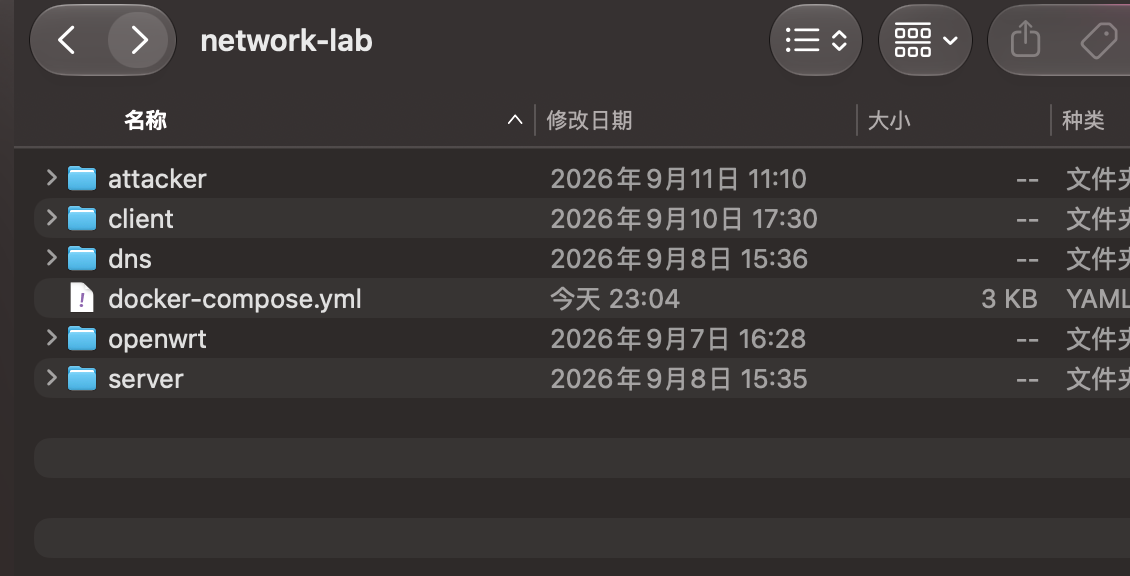
\includegraphics[width=0.8\textwidth]{figures/exp3_structure.png}
    \caption{实验配置目录}
\end{figure}

配置文件填写完之后，就可以开始部署
\begin{lstlisting}
docker compose up -d
\end{lstlisting}
如果想要进入某个机器，就用
\begin{lstlisting}
docker exec -it server bash
\end{lstlisting}
特别地,对于victim，我们利用远程桌面来连接
在主机浏览器访问https://localhost:6901,需要登录
\begin{figure}[H]
    \centering
    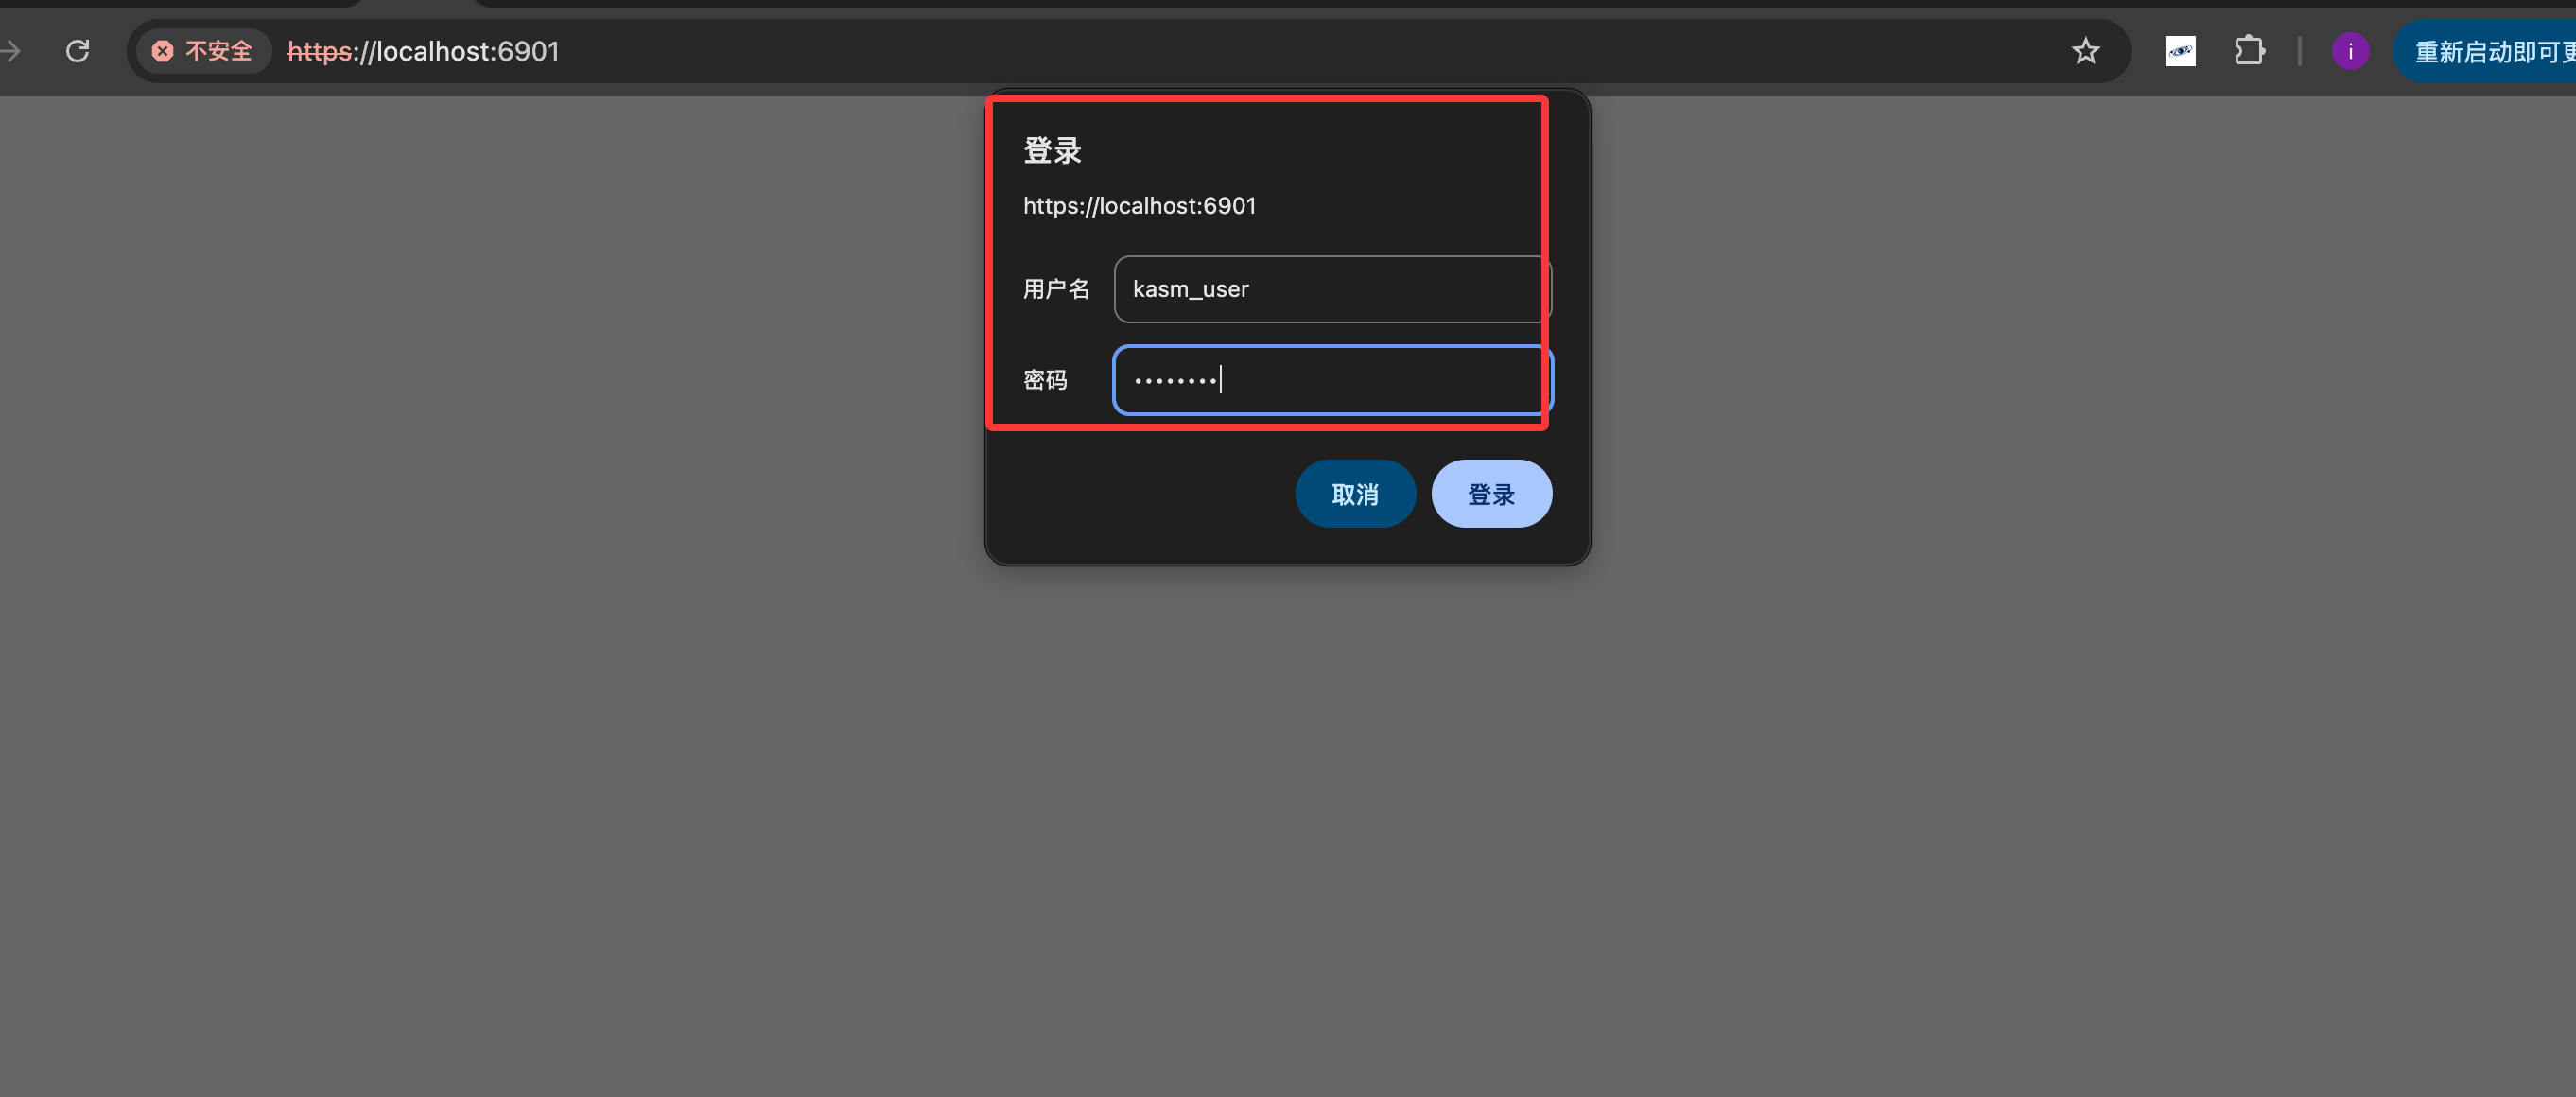
\includegraphics[width=0.8\textwidth]{figures/exp3_login.png}
    \caption{登录远程桌面}
\end{figure}
然后就就可以和其他虚拟机软件一样操控桌面端的ubuntu了,使用体验差距不大，比较方便的是直接同步了剪贴板
\begin{figure}[H]
    \centering
    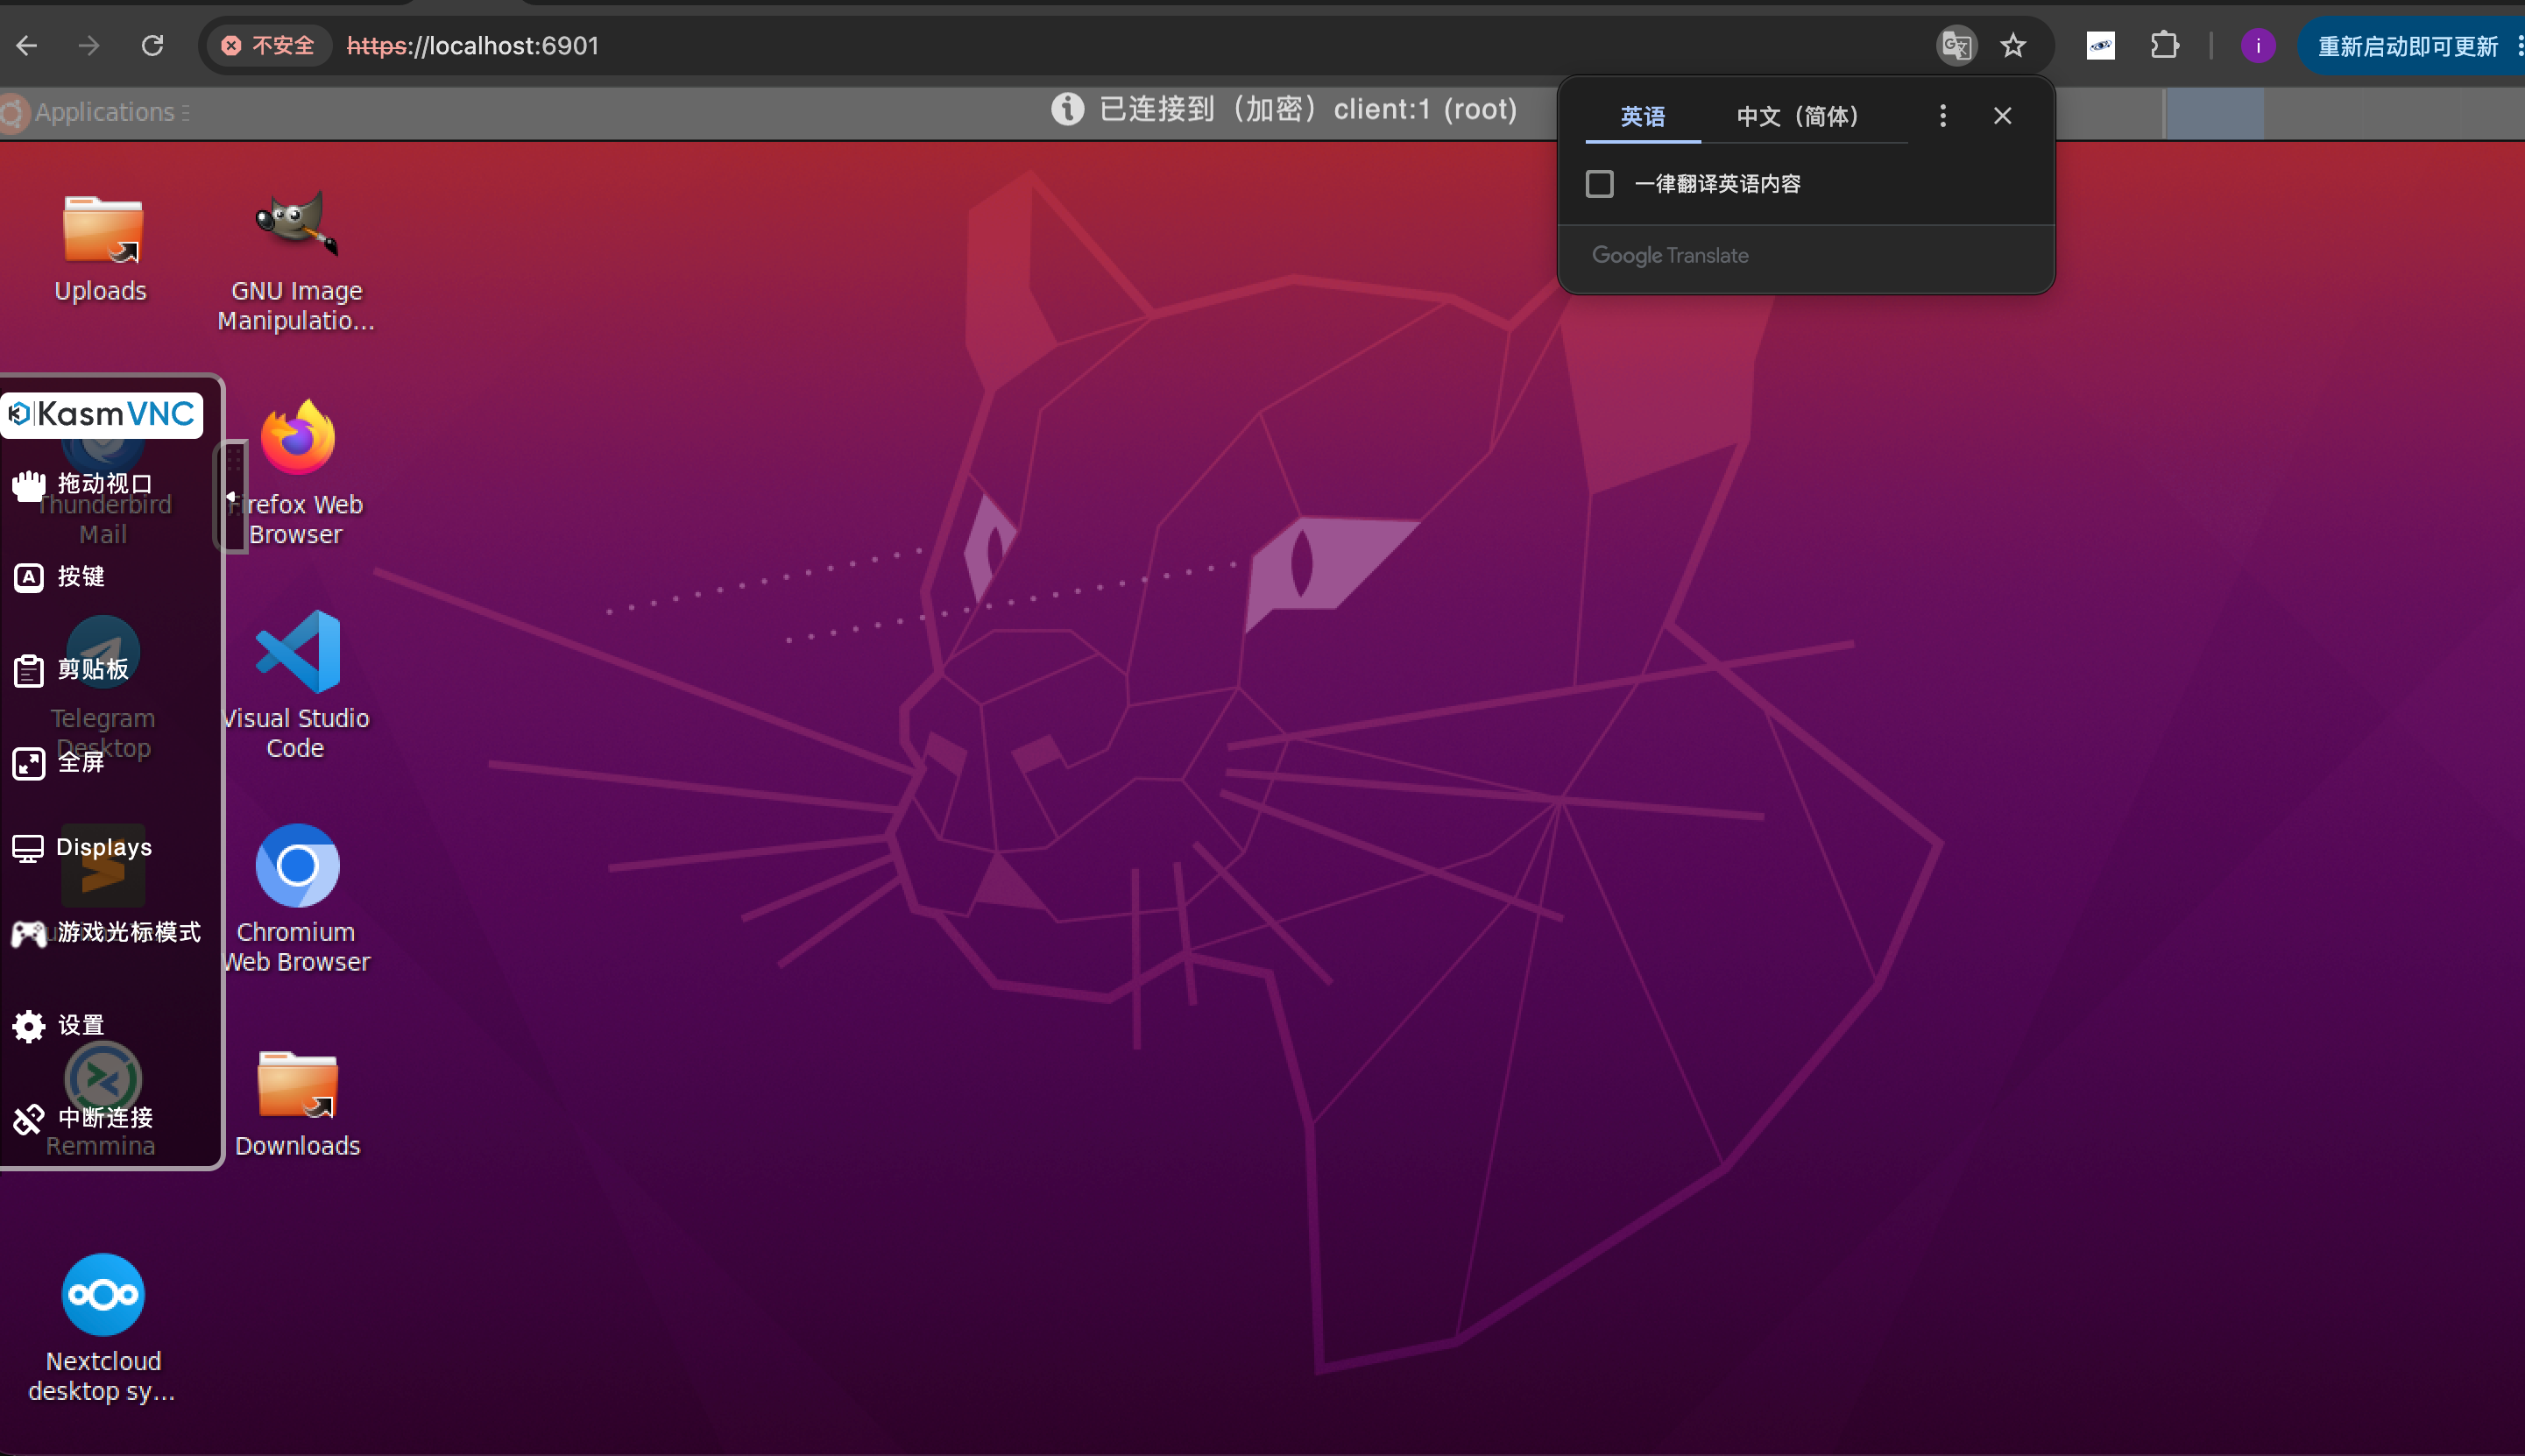
\includegraphics[width=0.8\textwidth]{figures/exp3_desktop.png}
    \caption{进入桌面}
\end{figure}
\begin{table}[H]
    \centering
    \caption{实验三各虚拟机网络接口及 IP 地址配置}
    \label{tab:exp3_network}
    \begin{tabular}{cccc}
        \toprule
        虚拟机 & Linux 内网卡名 & IP 地址 & 默认网关 \\
        \midrule
        Victim(Client)      & \texttt{eth0} & \texttt{192.168.3.10/24}  & \texttt{192.168.3.254} \\
        Attacker  & \texttt{eth0} & \texttt{192.168.2.100/24}  & \texttt{192.168.2.1} \\
        User  & \texttt{eth0} & \texttt{192.168.4.105/24} & \texttt{192.168.4.1} \\
        OpenWRT     & \texttt{eth0}   & \texttt{192.168.3.1/24}   & -- \\
        OpenWRT     & \texttt{eth1}   & \texttt{192.168.4.1/24}   & -- \\
        OpenWRT     & \texttt{eth2}   & \texttt{192.168.2.1/24}   & -- \\
        \bottomrule
    \end{tabular}
\end{table}
网络拓扑如图所示：
\begin{figure}[H]
    \centering
    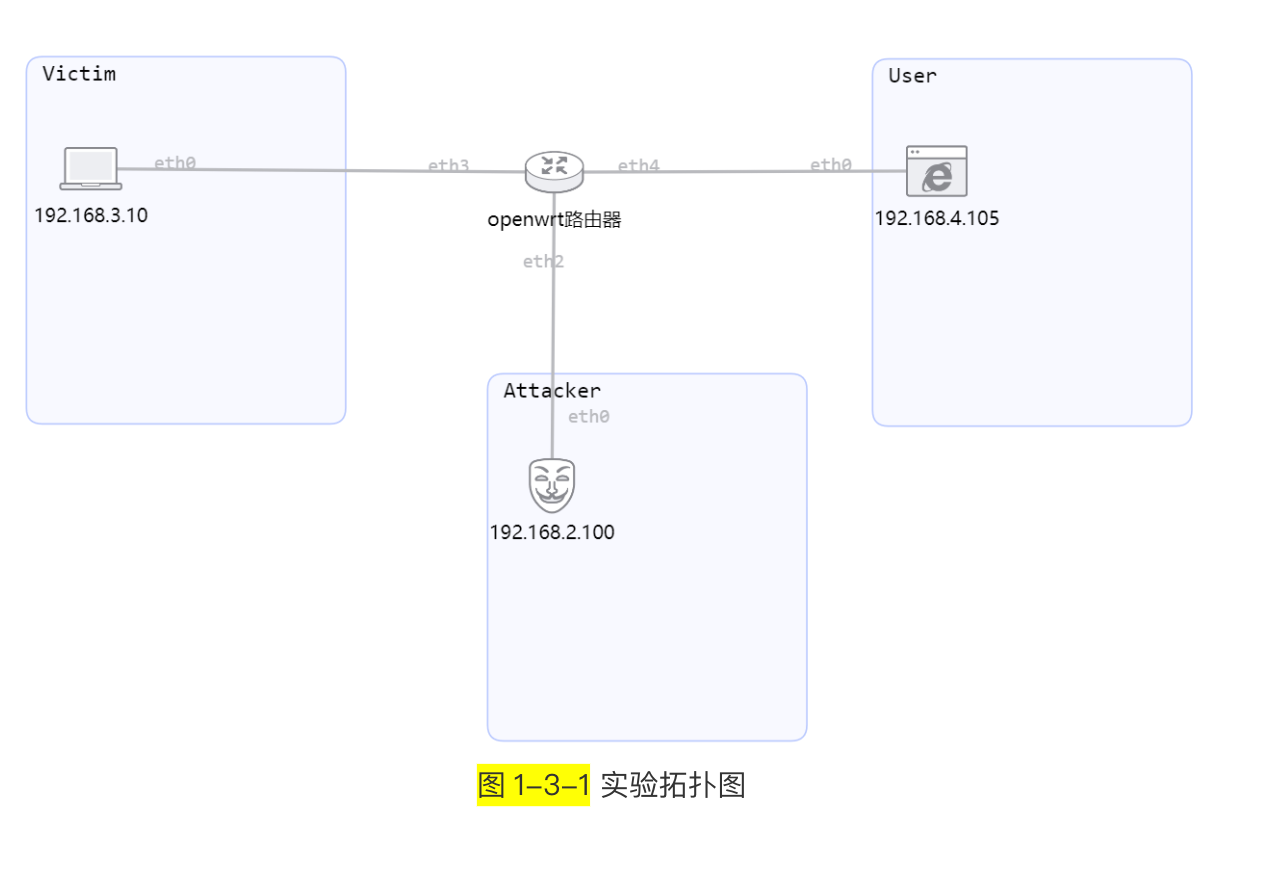
\includegraphics[width=0.8\textwidth]{figures/exp3_network.png}
    \caption{实验三网络拓扑图}
    \label{fig:exp3_network}
\end{figure}

\subsection{实验过程}
在 Attacker 上以 root 权限启动 Scapy：
\begin{figure}[H]
    \centering
    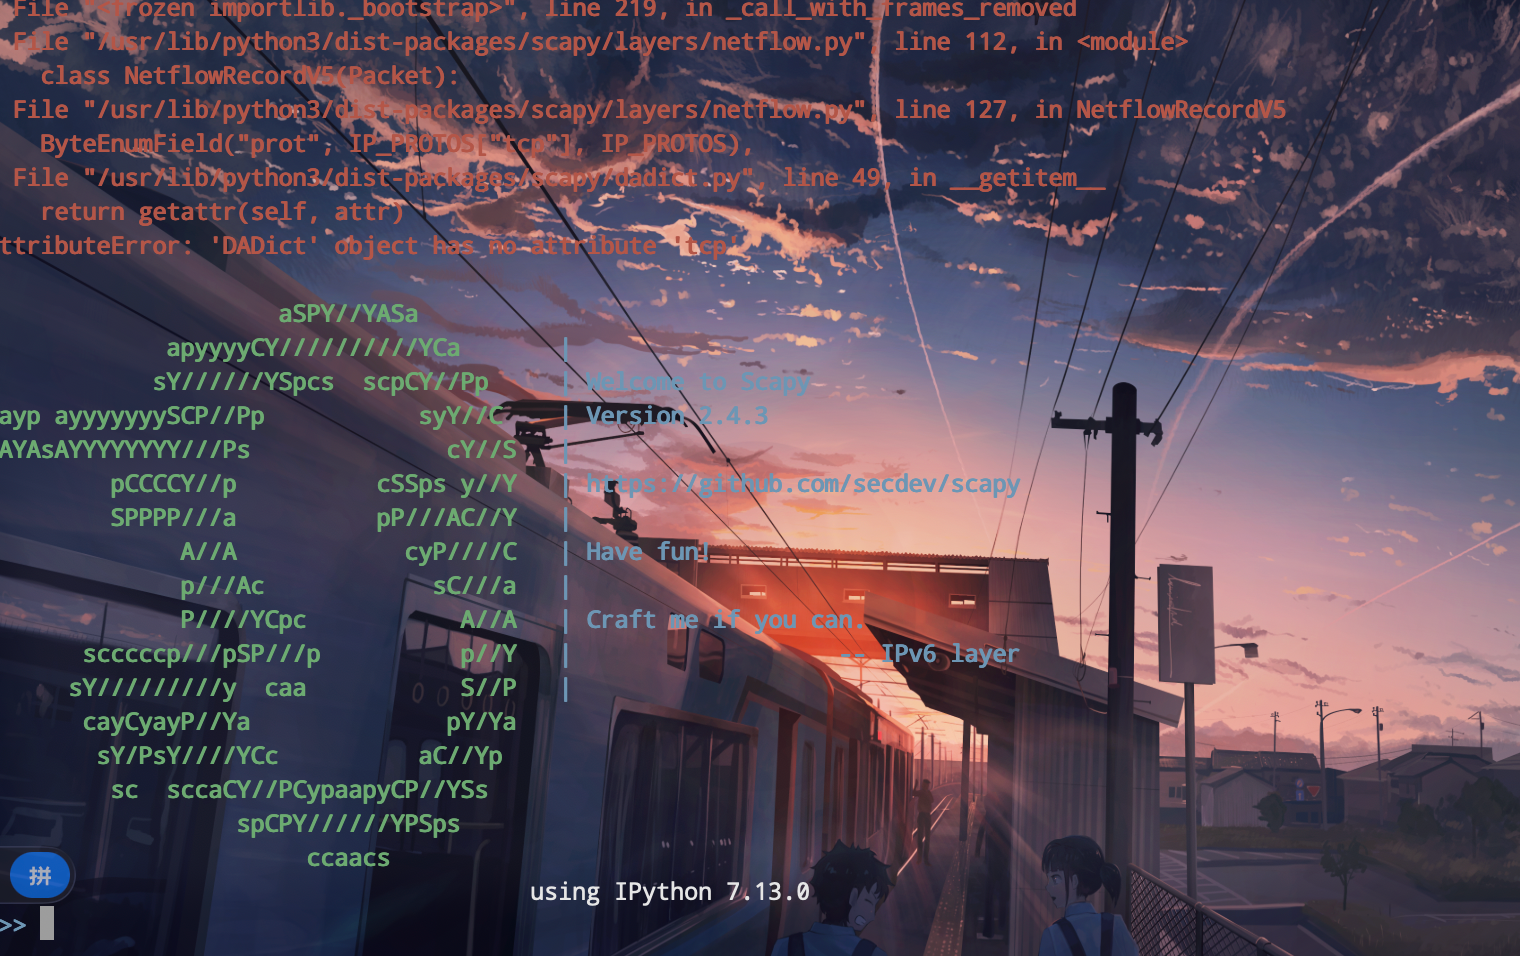
\includegraphics[width=0.8\textwidth]{figures/exp3_scapy.png}
    \caption{打开 Scapy}
    \label{fig:exp3_scapy}
\end{figure}
\subsubsection{创建ip层}
将源ip（src）设置为User ip，将目的ip（dst）设置成Victim ip；
\begin{lstlisting}[language=python]
ip_layer = IP(src="192.168.4.105", dst="192.168.3.10") 
\end{lstlisting}
通过 \texttt{ls(ICMP)} 查看 ICMP 层的默认字段值，其中 type=8 和 code=0 组合起来表示
ICMP Echo Request（Ping）数据包，未设置的字段将使用默认值填充。
\begin{figure}[H]
    \centering
    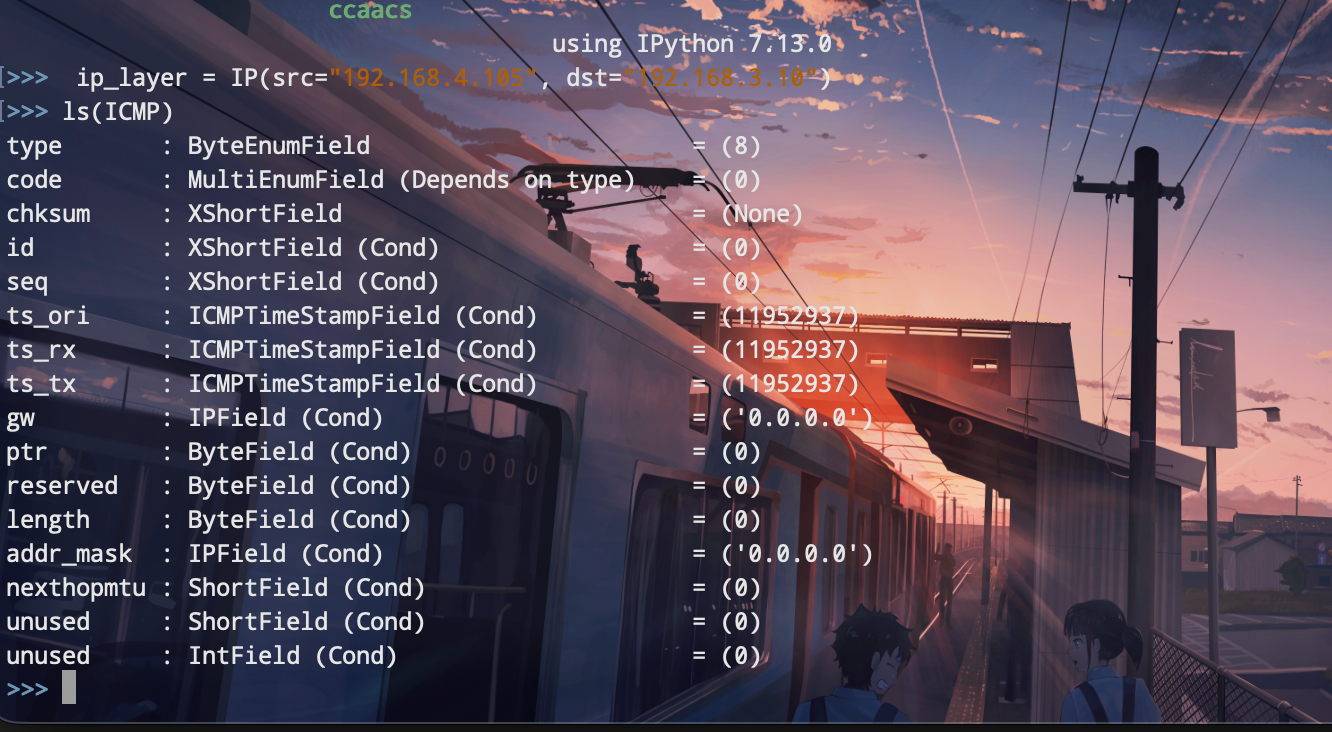
\includegraphics[width=0.8\textwidth]{figures/exp3_icmp.png}
    \caption{创建 IP 层、查看 ICMP 层}
    \label{fig:exp3_icmp}
\end{figure}
\subsubsection{创建 ICMP 层并添加负载}
\begin{lstlisting}[language=python]
icmp_layer = ICMP()  # 创建 ICMP 层
\end{lstlisting}
创建负载数据；
\begin{lstlisting}[language=python]
payload = "I come from Attacker-192.168.2.100"  # 负载内容
\end{lstlisting}
\subsubsection{构造 ICMP Echo Request 数据包}
将 IP 层、ICMP 层和 Raw 负载组合为一个 ICMP Echo Request 数据包；
\begin{lstlisting}[language=python]
icmp_request = ip_layer / icmp_layer / payload
\end{lstlisting}
通过 \texttt{show()} 方法查看已构造好的数据包内容；
\begin{figure}[H]
    \centering
    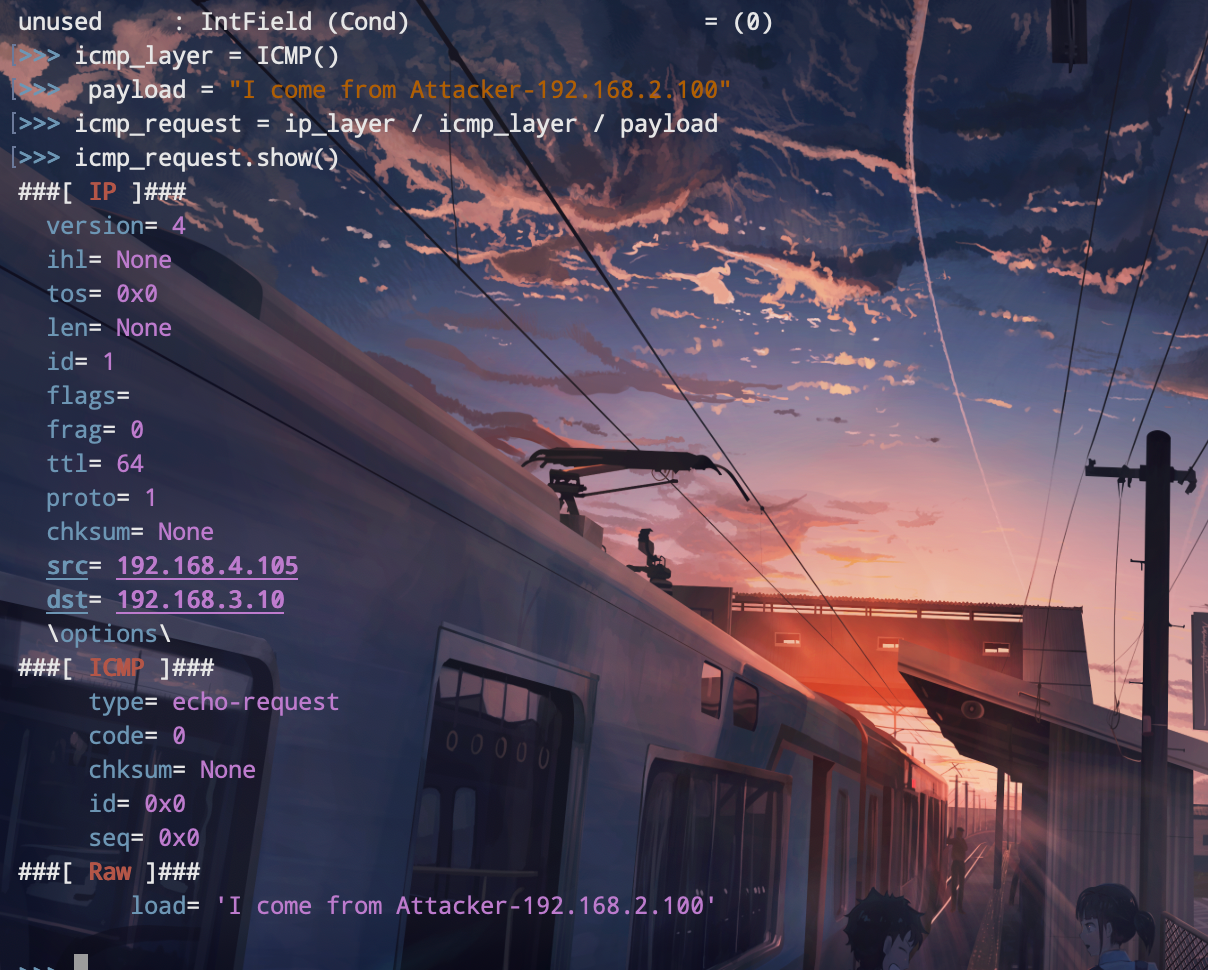
\includegraphics[width=0.8\textwidth]{figures/exp3_icmpcreate.png}
    \caption{创建 ICMP 层}
    \label{fig:exp3_icmpcreate}
\end{figure}
\subsubsection{发送数据包}
\begin{figure}[H]
    \centering
    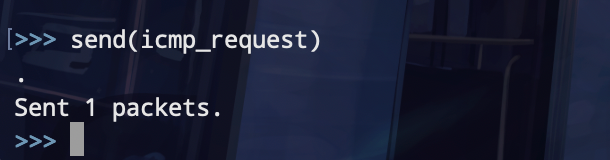
\includegraphics[width=0.8\textwidth]{figures/exp3_send.png}
    \caption{发送数据包}
    \label{fig:exp3_send}
\end{figure}
\subsubsection{收到数据包}
打开 Wireshark，监听 eth0 的流量，并过滤掉 6901 端口的流量，因为该端口用于远程桌面。
\begin{figure}[H]
    \centering
    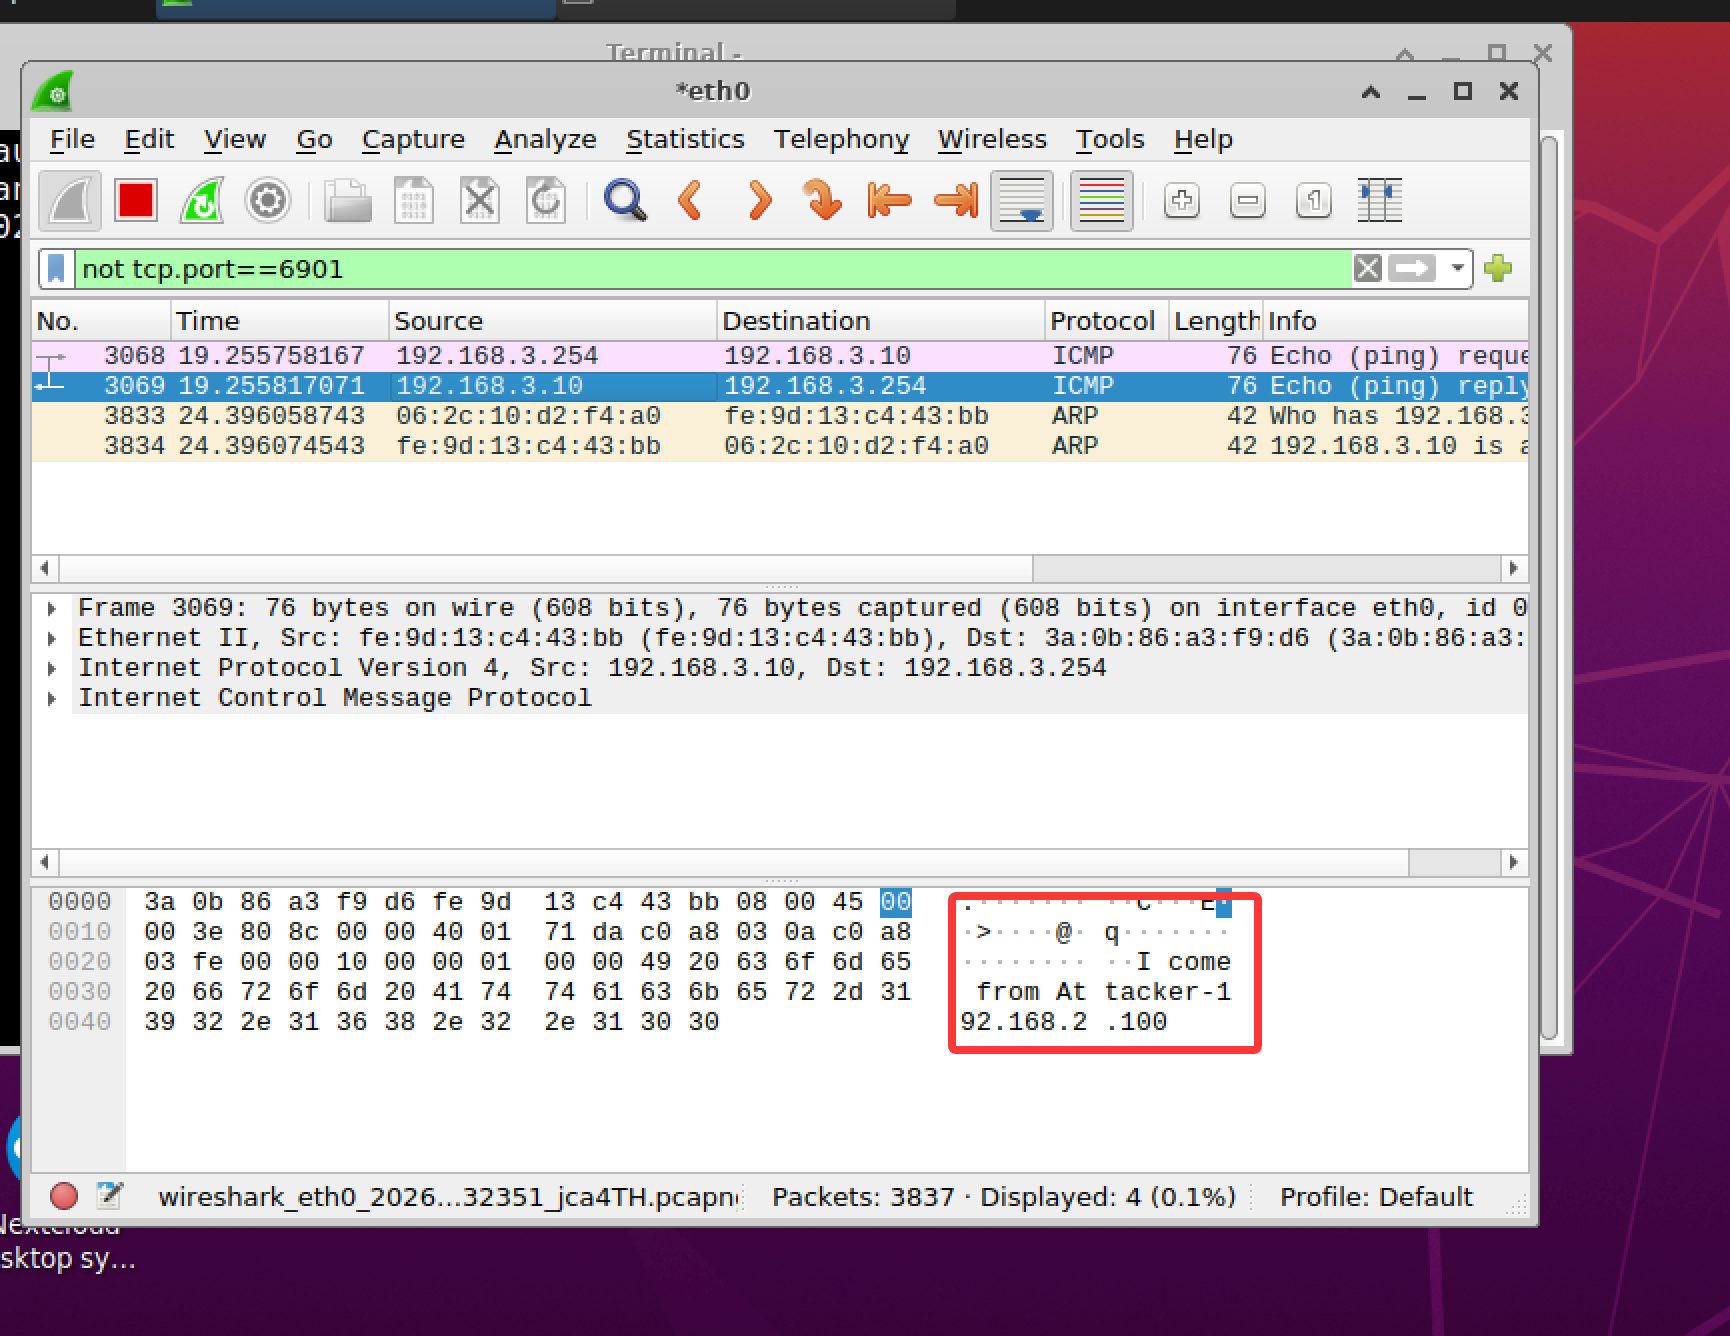
\includegraphics[width=0.8\textwidth]{figures/exp3_receive.png}
    \caption{收到数据包}
    \label{fig:exp3_receive}
\end{figure}
初次抓包时 Victim 看到的源地址是 192.168.3.254。这是因为 Docker 网络默认启用
IP masquerade，网关会将源 IP 地址替换为自身地址\cite{docker-bridge}。
\begin{figure}[H]
    \centering
    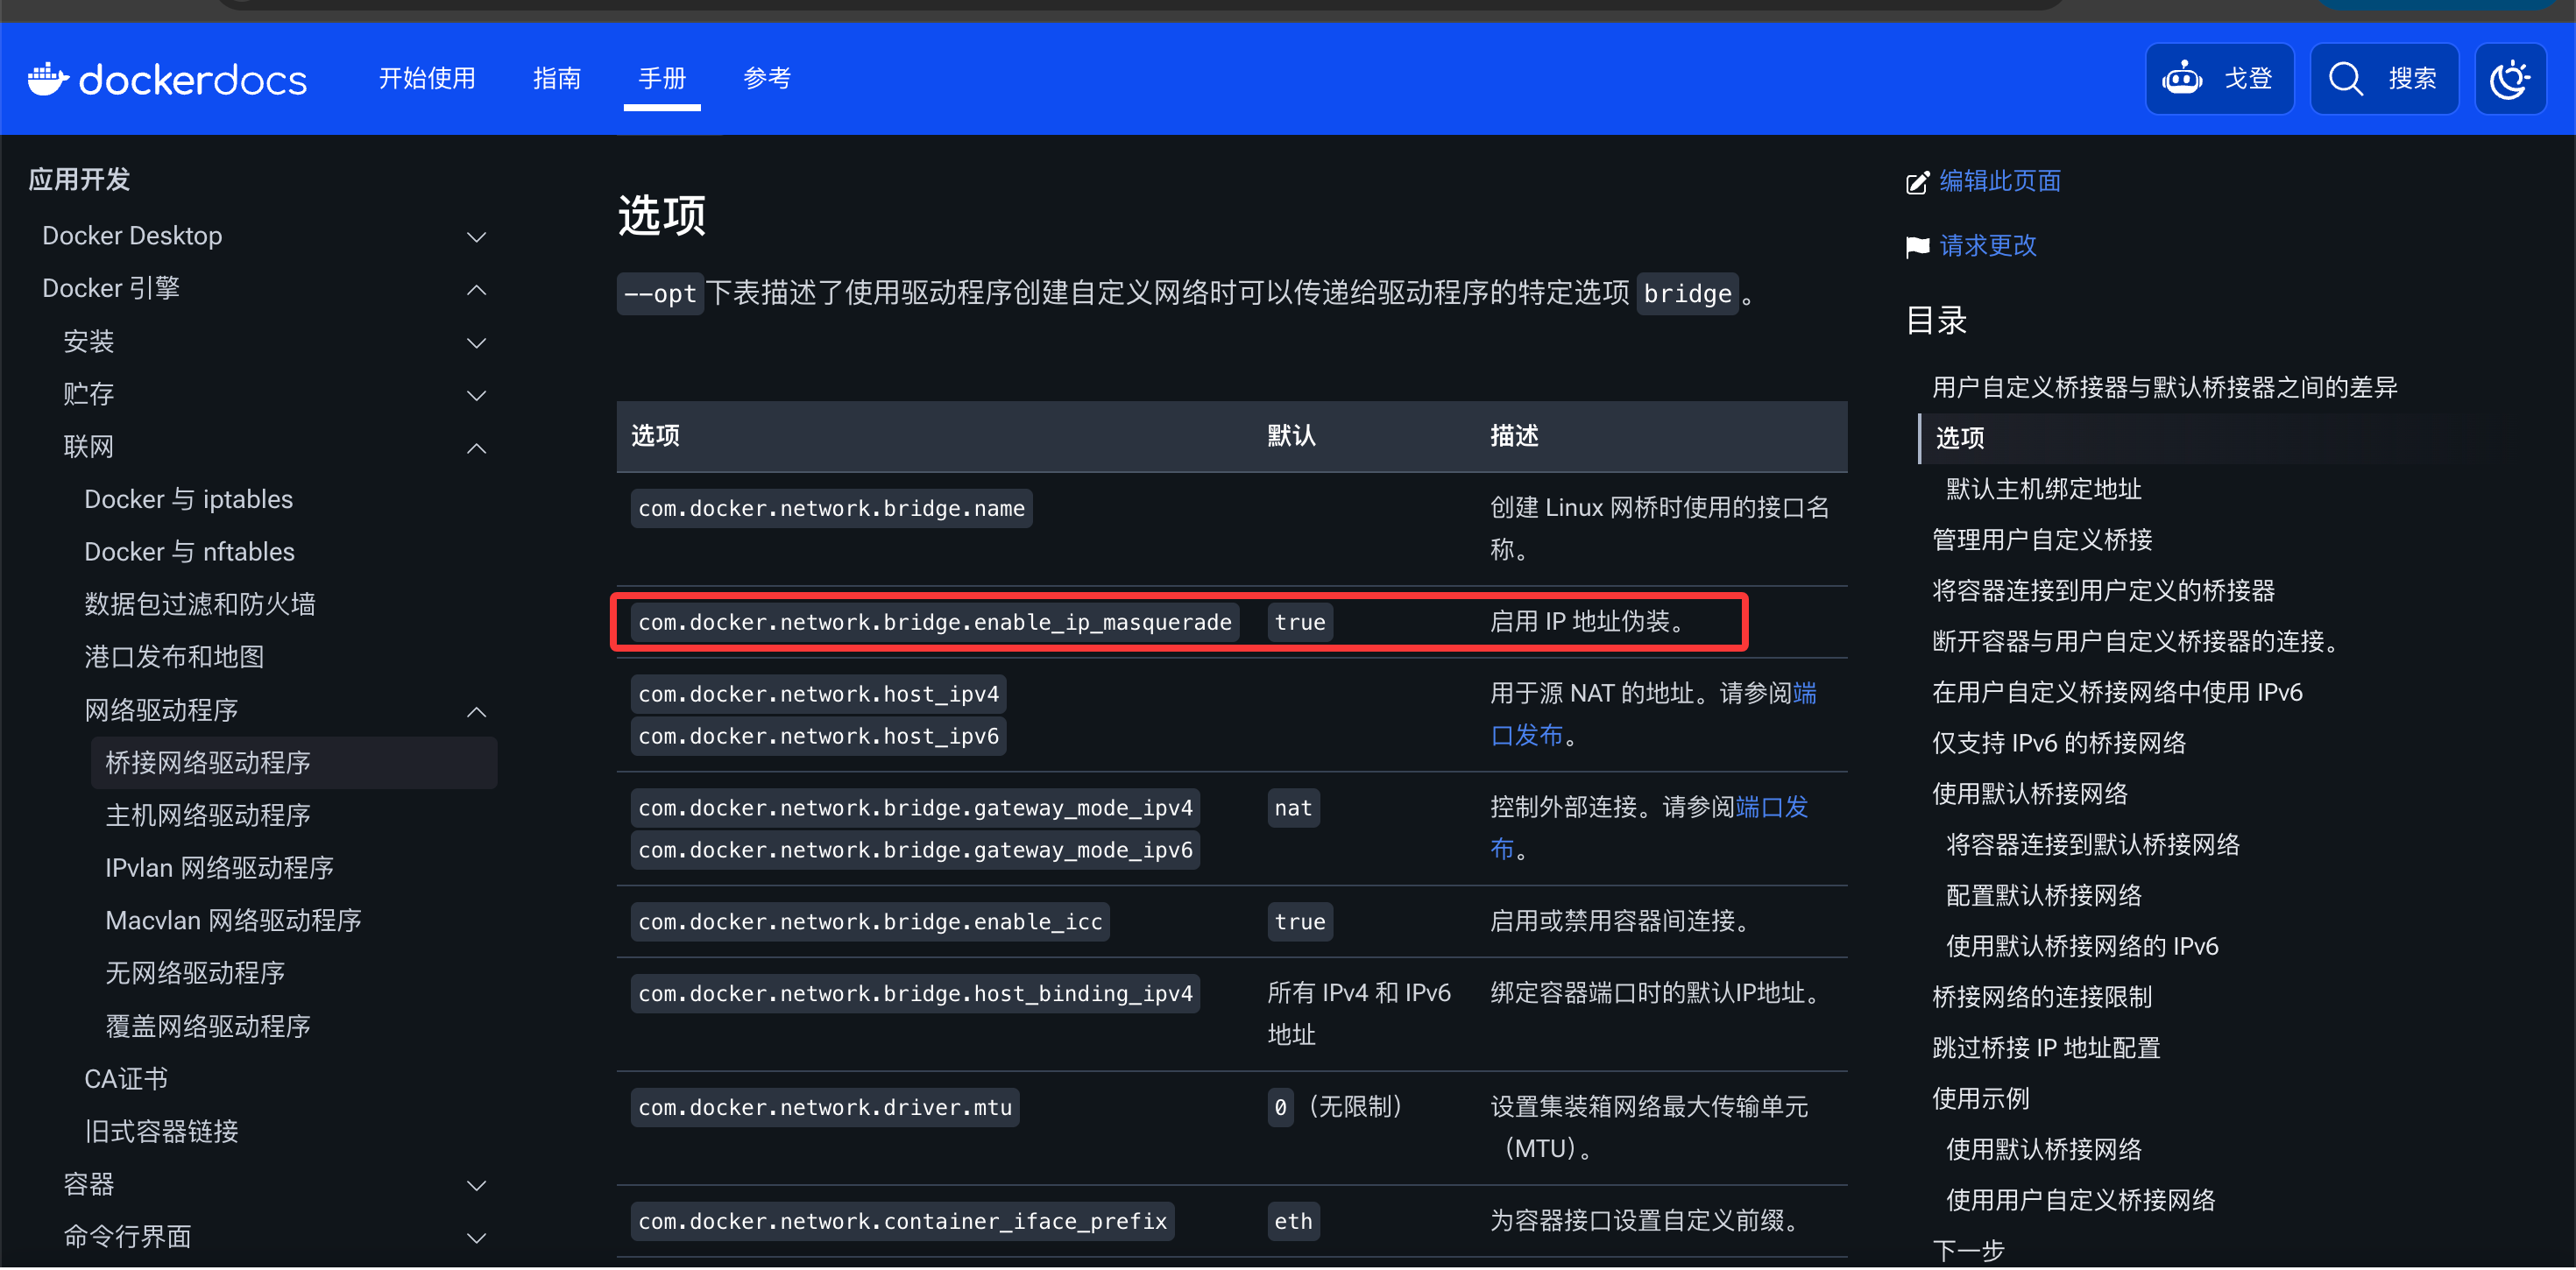
\includegraphics[width=0.8\textwidth]{figures/exp3_docker.png}
    \caption{Docker IP masquerade 现象}
\end{figure}
这会覆盖 Scapy 在 IP 首部中设置的源地址，因此需要在 docker-compose.yml 中关闭相关网络的
masquerade（附录中给出了修改后的配置）。
\begin{figure}[H]
    \centering
    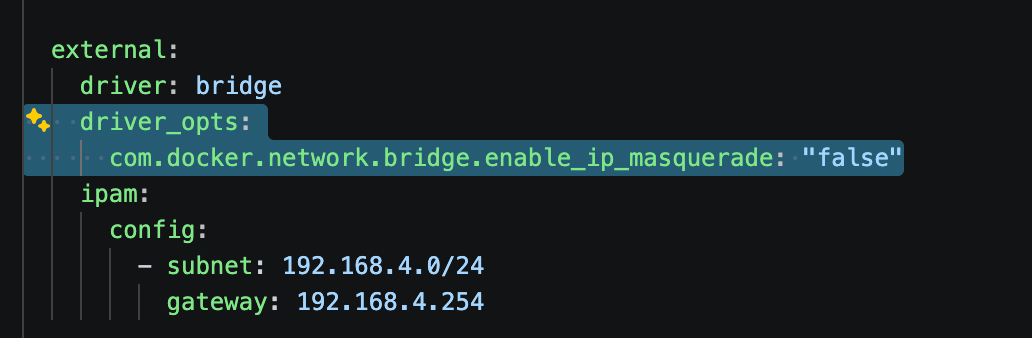
\includegraphics[width=0.8\textwidth]{figures/exp3_docker_revise.png}
    \caption{修改 docker-compose.yml}
\end{figure}
修改后重新发送，Victim 侧即可观察到 Scapy 构造的伪造源地址。
\begin{figure}[H]
    \centering
    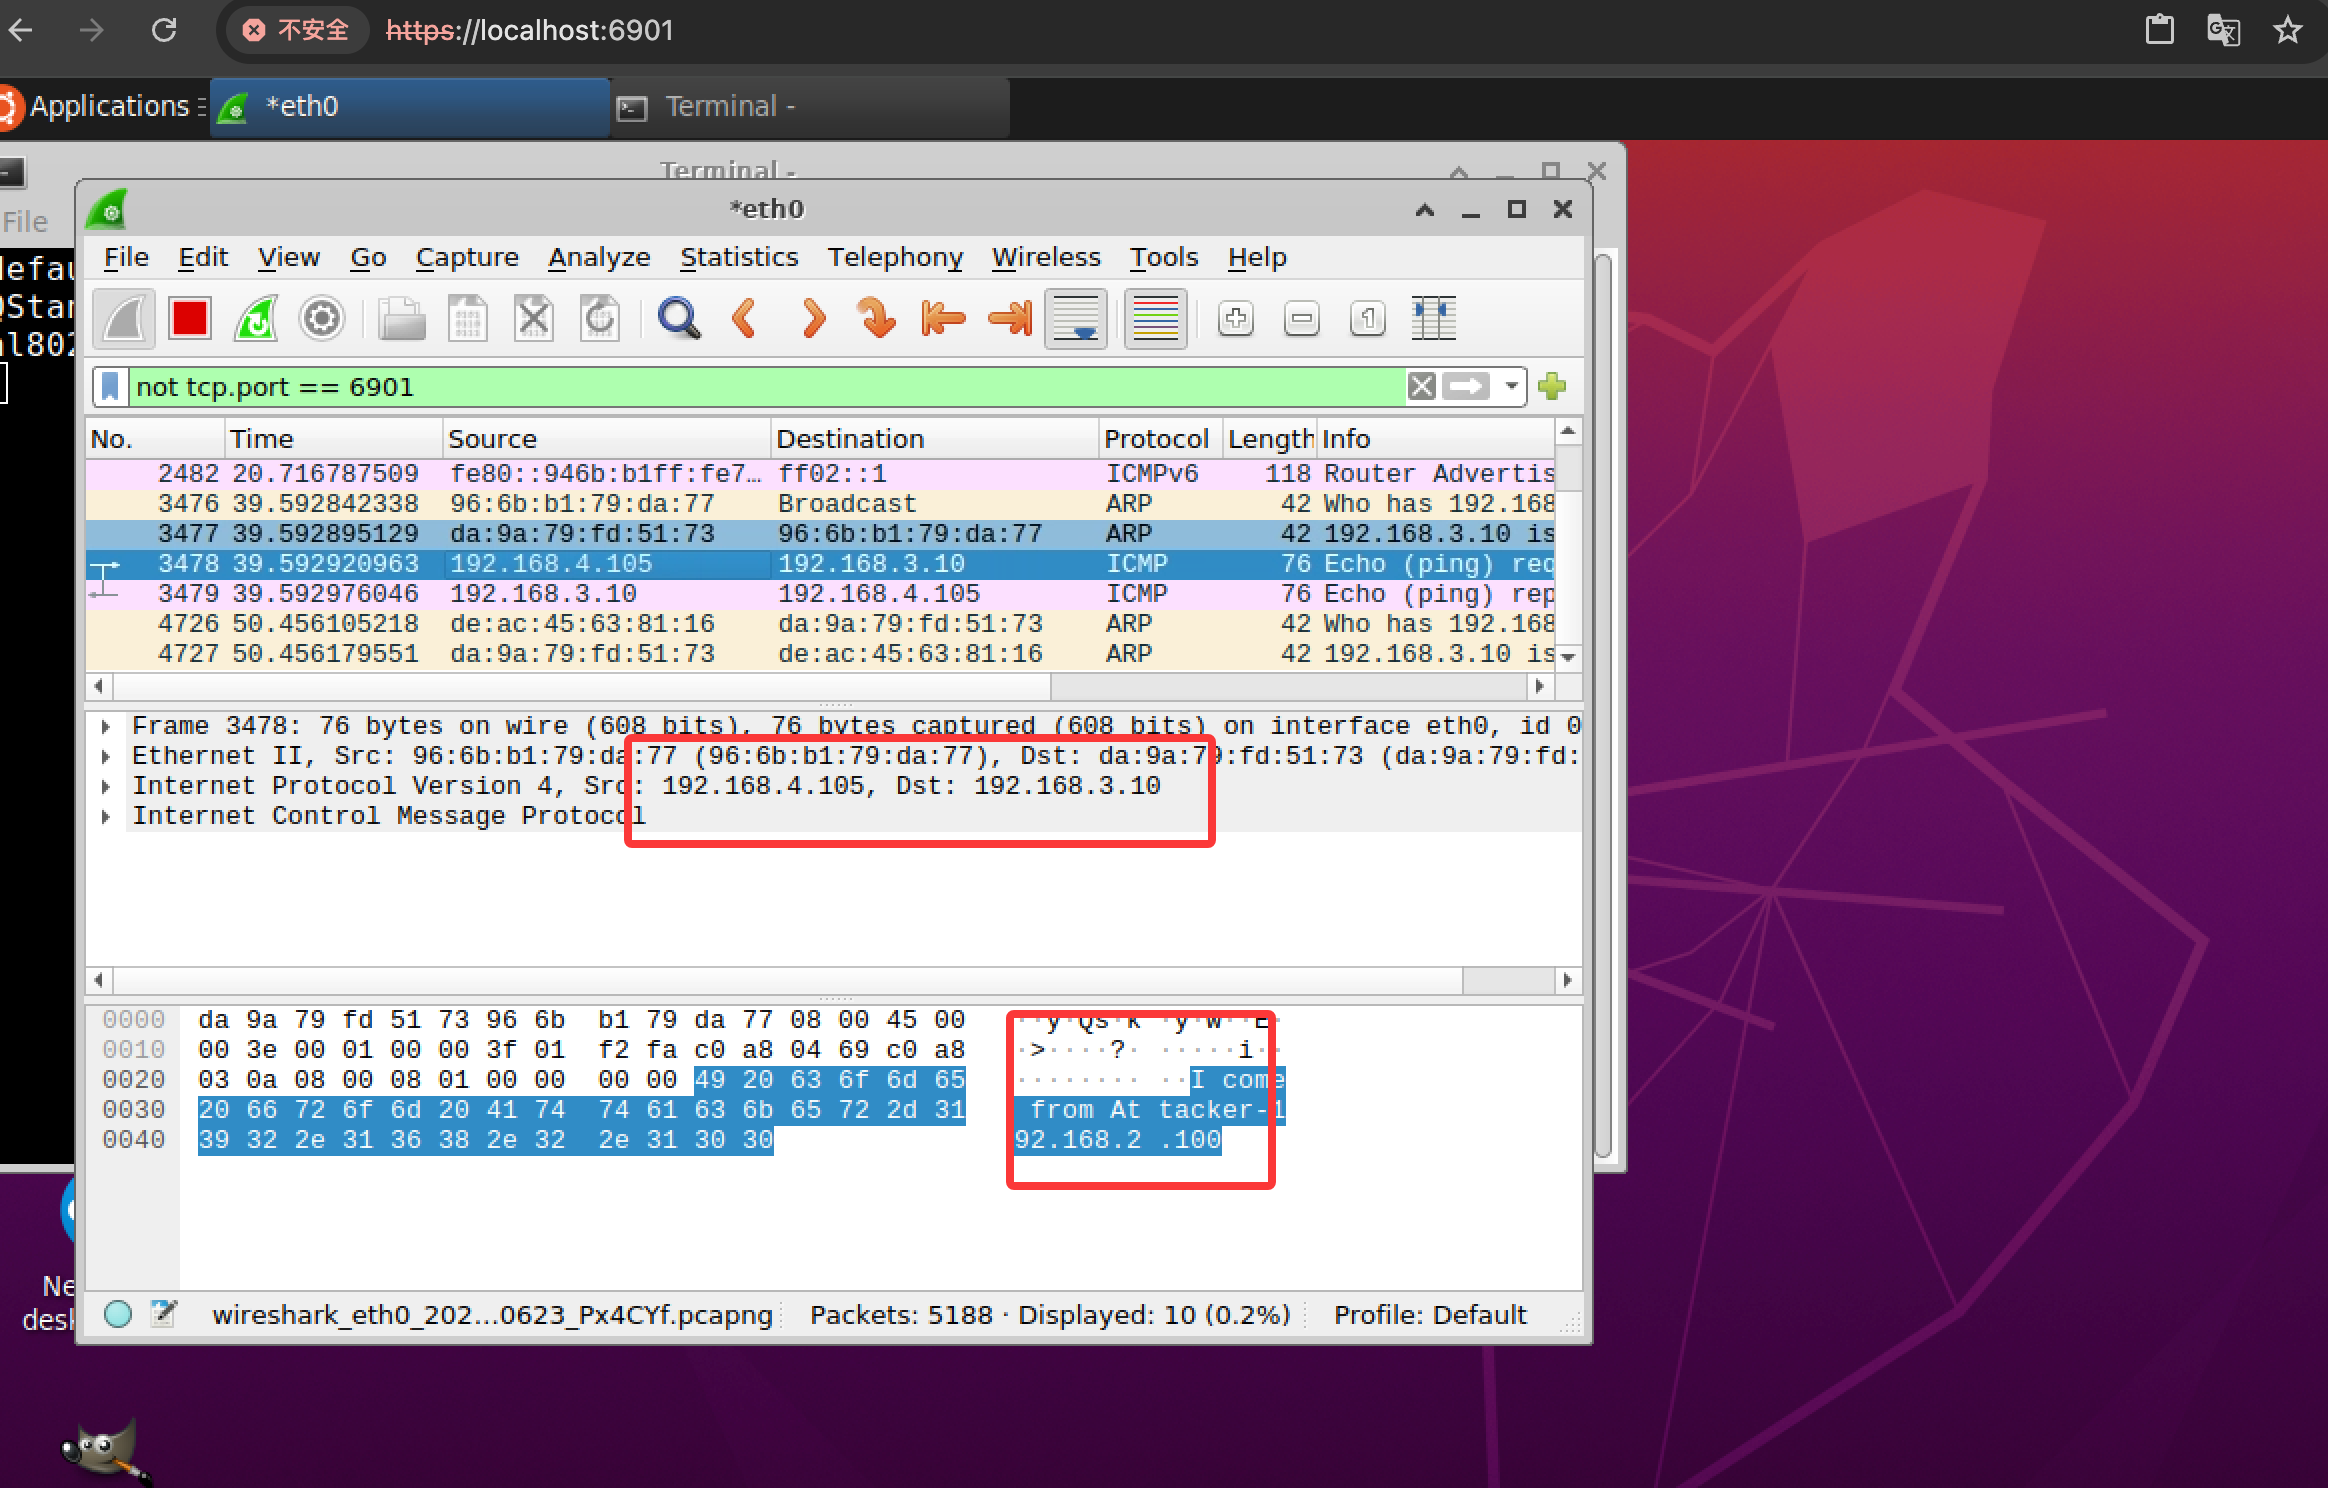
\includegraphics[width=0.8\textwidth]{figures/exp3_success.png}
    \caption{收到数据包}
\end{figure}
